\documentclass{beamer}
\title{HMM vs headache}
\usetheme{Copenhagen}
\usepackage{graphicx}
\usepackage{tikz}
\usetikzlibrary{positioning,arrows.meta,quotes}
\usetikzlibrary{shapes,snakes}
\usetikzlibrary{bayesnet}
\tikzset{>=latex}
\tikzstyle{plate caption} = [caption, node distance=0, inner sep=0pt,
below left=5pt and 0pt of #1.south]

\begin{document}
\frame{\titlepage}
\begin{frame}{Short description of the dataset and the problem}
The dataset contains a binary sequence of size 296. Each element has value 1 if in that they I had some headache and 0 if I had not. 
\end{frame}
\begin{frame}{Autocorrelation}
\includegraphics[scale=0.6]{acf}
First three lags are statistical significant, so it makes sense to model the data as a time series. We decide to use short memory HMM models.
\end{frame}
\begin{frame}{General model stucture}
${Z}_{t}$ Markov process with memory parametrized by $\theta$\\
${X}_{t}|Z_{t}=z_{t}\sim Ber(g(z_{t}))$ where $g:{A}\subseteq \mathbb{R}\rightarrow [0,1]$ eventually paramatrized by $\phi$ \\
$Z_{t}$ and $g$ characterize the model

 \begin{center}
    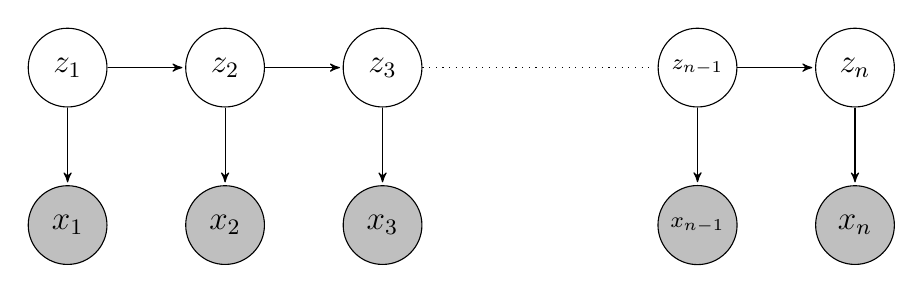
\begin{tikzpicture}[>=stealth', shorten >=1pt, auto,
    node distance=2.5cm, scale=1, 
    transform shape, align=center, 
    obs/.style={circle, draw=black, fill=lightgray,minimum size=1cm},
    state/.style={circle, draw=black, fill=white,minimum size=1cm}]s
    \centering
    \node [obs] (x_1) at (0,0) {\large $x_1$};
    \node [obs] (x_2) at (2,0) {\large $x_2$};
    \node [obs] (x_3) at (4,0) {\large $x_3$};
    \node [obs] (x_n-1) at (8,0) {\footnotesize $x_{n-1}$};
    \node [obs] (x_n) at (10,0) {\large $x_n$};
    
    \node [state] (z_1) at (0,2) {\large $z_1$};
    \node [state] (z_2) at (2,2) {\large $z_2$};
    \node [state] (z_3) at (4,2) {\large $z_3$};
    \node [state] (z_n-1) at (8,2) {\footnotesize $z_{n-1}$};
    \node [state] (z_n) at (10,2) {\large $z_n$};
    
    \path [draw,->] (z_1) edge (z_2);
    \path [draw,->] (z_2) edge (z_3);
    \path [draw, dotted] (z_3) edge (z_n-1);
    \path [draw,->] (z_n-1) edge (z_n);
    
    \path [draw,->] (z_1) edge (x_1);
    \path [draw,->] (z_2) edge (x_2);
    \path [draw, ->] (z_3) edge (x_3);
    \path [draw,->] (z_n-1) edge (x_n-1);
    \path [draw,->] (z_n) edge (x_n);

    \end{tikzpicture}
 \end{center}
\end{frame}
\begin{frame}{Model 1}
\begin{block}{Wiener Process}
$Z_{t}$ is a Wiener process if:
\begin{itemize}
\item$Z_{t}\sim N(0,t)$
\item $Cov(Z_{t},Z_{s})=min\{t,s\}$
\end{itemize} 
\end{block}
Our first model consists of:
\begin{itemize}
\item $Z_{t}$ Wiener process
\item $g(z)=e^{-\phi z^{2}}$  
\end{itemize}
We can prove that given $S=\{ i | x_{i}=1\}$ $p(x)=\sqrt{\frac{1}{1+\phi\sum\limits_{i \in 1...N \backslash S} i}}-\sum \limits _{D\subset S} \sqrt{\frac{1}{1+\phi\sum \limits_{i \in 1...N \backslash D} i}}$
\\Howewer the cardinality of the power set is $2^{|S|}$ so it is computationally unfeasible even if we have an analytical form. For this reason it is better to use approximation methods like SVI.
\end{frame}
\begin{frame}{Model 1}
For SVI we chosen $q_{\theta}(x)$ as a $Beta(\alpha,\beta)$.  The optimal $\phi$ is $2.69$.
\end{frame}
\end{document}